\documentclass[a4paper]{beamer}
\usepackage[spanish]{babel}
\usepackage[utf8]{inputenc}
\usepackage{graphicx}
\usepackage{biblatex}
\usepackage{enumerate}
\usepackage{csquotes}
\usepackage{braket}
\usepackage{amsmath}
\usepackage{pifont}

\title{Modos rotacionales y vibracionales en moléculas}
\author{José Soto García}
\begin{document}
\maketitle
%DIAPOSITIVA 1
\begin{frame}{La molécula como un sólido rígido}
\begin{itemize}
\item Suponemos la molécula como un sólido rígido.
\item La vibración ocurre en una escala temporal mucho menor que las rotaciones.
\item En una rotación los átomos vibran tantas veces que podemos considerar que estan quietos en su posición de equilibrio.
\item Consideramos la distancia interatómica como la distancia media $\braket{R}$.	
\end{itemize}
\end{frame}
%DIAPOSITIVA 2
\begin{frame}{La molécula como un sólido rígido}
\framesubtitle{Un poco de mecánica clásica}
  Para un sólido poliatómico se define el tensor de inercia $\tilde I$ como:
  \[\small{
\tilde{I}=\begin{pmatrix}
\displaystyle\sum_{\alpha}m_{\alpha}\left(x^2_{\alpha,2}+x^2_{\alpha,3}\right) & -\displaystyle\sum_{\alpha}m_{\alpha}x_{\alpha,1}x_{\alpha,2} & -\displaystyle\sum_{\alpha}m_{\alpha}x_{\alpha,1}x_{\alpha,3} \\\\
-\displaystyle\sum_{\alpha}m_{\alpha}x_{\alpha,2}x_{\alpha,1} & \displaystyle\sum_{\alpha}m_{\alpha}\left(x^2_{\alpha,1}+x^2_{\alpha,3}\right) &-\displaystyle\sum_{\alpha}m_{\alpha}x_{\alpha,2}x_{\alpha,3} \\\\
-\displaystyle\sum_{\alpha}m_{\alpha}x_{\alpha,3}x_{\alpha,1} & -\displaystyle\sum_{\alpha}m_{\alpha}x_{\alpha,3}x_{\alpha,2} & \displaystyle\sum_{\alpha}m_{\alpha}\left(x^2_{\alpha,1}+x^2_{\alpha,2}\right) \end{pmatrix}}
\]

La energía cinética rotacional del sistema se obtiene como
$$T_{rot}=\frac{1}{2}\sum_{i,j}I_{ij}\omega_i\omega_j$$

\end{frame}

%DIAPOSITIVA 3
\begin{frame}{La molécula como un sólido rígido}
\framesubtitle{Un poco de mecánica clásica}
Si diagonalizamos el tensor de inercia
$$\tilde I = \begin{pmatrix}
I_a & 0 & 0\\
0 & I_b & 0\\
0 & 0 & I_c
\end{pmatrix}$$

$$T_{rot}=\frac{1}{2}\left(I_a\omega^2_a + I_b\omega^2_b + I_c\omega^2_c\right)$$
 Para formar el hamiltoniano del sistema necesitamos la energía en función del momento angular $\boldsymbol P$ con $P_i=I_i\omega_i$ 
 $$T_{rot}=\frac{P_a^2}{2I_a}+\frac{P_b^2}{2I_b}+\frac{P_c^2}{2I_c}$$
\end{frame}

%DIAPOSITIVA 4
\begin{frame}{La molécula como un sólido rígido}
\begin{equation*}
\hat H_{rot}=\frac{\hat P_a^2}{2I_a}+\frac{\hat P_b^2}{2I_b}+\frac{\hat P_c^2}{2I_c}
\end{equation*}
\framesubtitle{Pasamos a la cuántica}
\begin{figure}
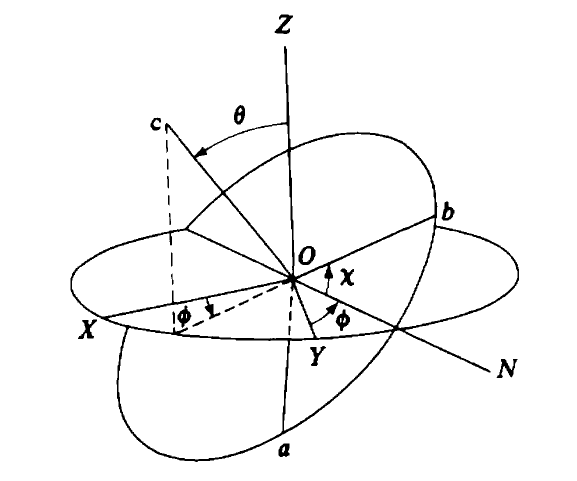
\includegraphics[width=0.4\textwidth]{Angulos_Euler.png}
\caption{Ángulos de Euler. }
\label{euler}
\end{figure}
$$
\hat P_{\phi}=-i\hbar\frac{\partial}{\partial \phi},\,\ \hat P_{N}=-i\hbar\frac{\partial}{\partial N},\,\ \hat P_{\chi}=-i\hbar\frac{\partial}{\partial \chi}
$$
\end{frame}

%DIAPOSITIVA 5
\begin{frame}{La molécula como un sólido rígido}
\framesubtitle{Pasamos a la cuántica}
Con un poco de trigonometría
\begin{equation*}
{\tiny\hat P_a = i\hbar \left[cos\chi csc\theta \frac{\partial}{\partial \phi} - cos\chi cot\theta \frac{\partial}{\partial \chi} - sin\chi \frac{\partial}{\partial \theta} \right]}
\end{equation*}
\begin{equation*}
\tiny\hat P_b = i\hbar \left[-sin\chi csc\theta \frac{\partial}{\partial \phi} + sin\chi cot\theta \frac{\partial}{\partial \chi} - cos\chi \frac{\partial}{\partial \theta} \right]
\end{equation*}
\begin{equation*}
\tiny\hat P_c = -i\hbar \frac{\partial}{\partial\chi}
\end{equation*}

O también:

\begin{equation*}
\hat P_X = i\hbar \left[cos\phi cot\theta \frac{\partial}{\partial \phi} - cos\phi csc\theta \frac{\partial}{\partial \chi} + sin\phi \frac{\partial}{\partial \theta} \right]
\end{equation*}
\begin{equation*}
\hat P_Y = i\hbar \left[sin\phi cot\theta \frac{\partial}{\partial \phi} - sin\phi csc\theta \frac{\partial}{\partial \chi} - cos\phi \frac{\partial}{\partial \theta} \right]
\end{equation*}
\begin{equation*}
\hat P_Z = -i\hbar\frac{\partial}{\partial\phi} 
\end{equation*}
\end{frame}

%DIAPOSITIVA 6
\begin{frame}{La molécula como un sólido rígido}
\framesubtitle{¿Cómo obtenemos las autofunciones y autoenergías del hamiltoniano?}
\begin{itemize}
\item	Sustituiyendo $\hat P_a$, $\hat P_b$ y $\hat P_c$ en $\hat H_{rot}$ y resolviendo la ecuación de autovalores \ding{55}
\item Usando relaciones de conmutación \ding{51}
\begin{equation*}
\left[H_{rot}, \hat P^2 \right] = 0
\end{equation*}
\begin{equation*}
\left[H_{rot}, \hat P_J \right] = 0
\end{equation*}
\begin{equation*}
\left[H_{rot}, \hat P_c \right] = i\hbar \left(\frac{1}{2I_a}-\frac{1}{2I_b}\right)\left(\hat{P_a}\hat{P_b}+\hat{P_b}\hat{P_a}\right)
\end{equation*}
\end{itemize}
Lo que nos da 
\begin{equation}
\hat H\psi = E\psi
\end{equation}
\begin{equation}
\hat P^2\psi = J(J+1)\hbar \psi, \qquad J=0,1,2...
\end{equation}
\begin{equation}
\hat P_Z\psi = M\hbar\psi, \qquad M = 0,\pm 1,...,\pm J
\end{equation}
\end{frame}

%DIAPOSITIVA 7
\begin{frame}{Rotor rígido cuántico: Estados propios y autovalores}
\framesubtitle{El rotor esférico $I_a=I_b=I_c= I$}
La ecuación de Schödinger es:
\begin{equation*}
\frac{\hat P^2}{2I} \psi = E\psi
\end{equation*}
Resolviendo la ecuación obtenemos que:$$\frac{1}{2I}J(J+1)\hbar^2\psi=E\psi$$
\begin{equation}
E=\frac{J(J+1)\hbar^2}{2I}, \qquad J=0,1,2...
\end{equation}
En este caso, tenemos además que
\begin{equation}
\left[\hat H,\hat P_c \right]=0
\end{equation}
con $$\hat P_c \psi = K\hbar\psi, \qquad K = 0, \pm 1,..., \pm J$$
Luego la energía está $(2J+1)^2$ veces degenerada.
\end{frame}

%DIAPOSITIVA 8
\begin{frame}{Rotor rígido cuántico: Estados propios y autovalores}
\framesubtitle {El rotor simétrico: $I_a=I_b\neq I_c$ (caso achatado) o $I_a\neq I_b=I_c$ (caso alargado)}
La ecuación de Schrödinger es
\begin{equation*}
\frac{\hat P^2- \hat P_c^2}{2I_b}+\frac{\hat P_c^2}{2I_c}\psi=E\psi
\end{equation*}
En este caso también tenemos que:
\begin{equation}
\left[\hat H,\hat P_c \right]=0
\end{equation}
Luego llamando:
 \begin{equation}
 A \equiv \frac{h}{8\pi^2I_a}\geq B\equiv \frac{h}{8\pi^2I_b}\geq C\equiv \frac{h}{8\pi^2I_c}
 \end{equation}
 Llegamos a que:
 \begin{equation}
 E/h=BJ\left(J+1\right)+\left(C-B\right)K^2 \qquad (achatado)
 \end{equation}
 \begin{equation}
 E/h=BJ\left(J+1\right)+\left(A-B\right)K^2 \qquad (alargado)
 \end{equation}
 Y la energía está $4j+2$ veces degenerada
\end{frame}

%DIAPOSITIVA 9
\begin{frame}{Rotor rígido cuántico: Estados propios y autovalores}
\framesubtitle {El rotor asimétrico: $I_a \neq I_b\neq I_c$ }
En este caso
\begin{equation}
\left[\hat H,\hat P_c \right] \neq 0
\end{equation}
Y el hamiltoniano no es separable.
Podemos resolver la ecuación del hamiltoniano usando  las autofunciones del rotor simétrico
\begin{equation}
\psi_i = \sum_{K'=-J}^Jc_{i,JMK'}\phi_{JMK'}
\end{equation}
con
\begin{equation}
H_{K'K''}\equiv\int\phi^*_{JMK'}\hat H\phi_{JMK''}d\tau
\end{equation}
Y sus autofunciones son de la forma
\begin{equation}
\psi_i = \sum_{K'=-J}^Jc_{i,JMK'}\phi_{JMK'}
\end{equation}
\end{frame}

%DIAPOSITIVA 10
\begin{frame}{Estructura del espectro rotacional}
\begin{itemize}
\item Región de microondas
\item Sólo moléculas con momento dipolar eléctrico permanente
\item Acoplamiento frecuencia magnética irradiada con frecuencia del dipolo
\item Reglas de selección: $\bra{\psi_{JMK}}\hat D \ket{\psi_{J'K'M'}}$
\begin{equation*}
\Delta J = 0,\pm 1 \qquad\Delta K =0 \qquad \Delta M = 0, \pm 1
\end{equation*}
\item Intensidad absorción $\propto$ probabilidad ocupación de los niveles
\begin{equation*}
\frac{N_J}{N_0}=(2J+1)e^{-BhJ(J+1)/kT}
\end{equation*}
\end{itemize}
\begin{figure}
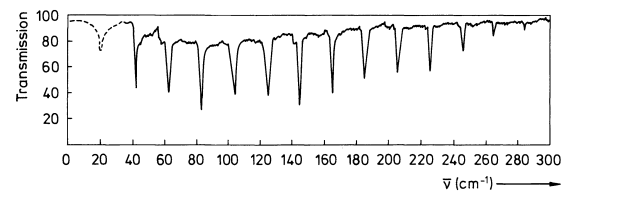
\includegraphics[width=0.6\textwidth]{intensidad.png}
\caption{Espectro rotacional para el HCl en estado gaseoso.}
\label{intensidad}
\end{figure}
\end{frame}

%DIAPOSITIVA 11
\begin{frame}{Algunos ejemplos}
\framesubtitle{$H_2$}
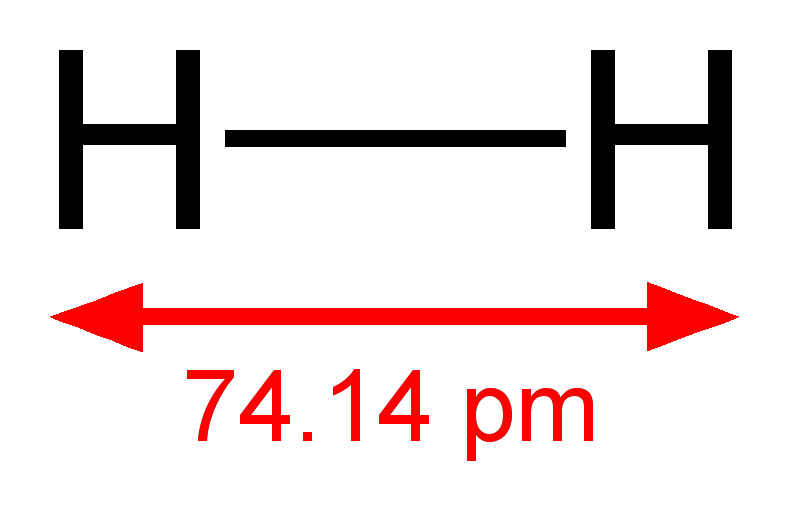
\includegraphics[width=0.3\textwidth]{hidrogeno.png}\\
$$I=\frac{1}{2}mR^2$$
 $R=74 \, pm=375.014 \, MeV^{-1}$\\
 $m=938.272 \, MeV/c^2$\\
 \begin{itemize}
  \item Nos queda que 
 $$I=65.977 \, eV^{-1}c^{-2}$$
\item luego 
 $$E_{rot} = 7.58\cdot 10^{-3}J(J+1)\, eV$$
 \end{itemize}
\end{frame}

%DIAPOSITIVA 12
\begin{frame}{Algunos ejemplos}
\framesubtitle{$CH_4$}
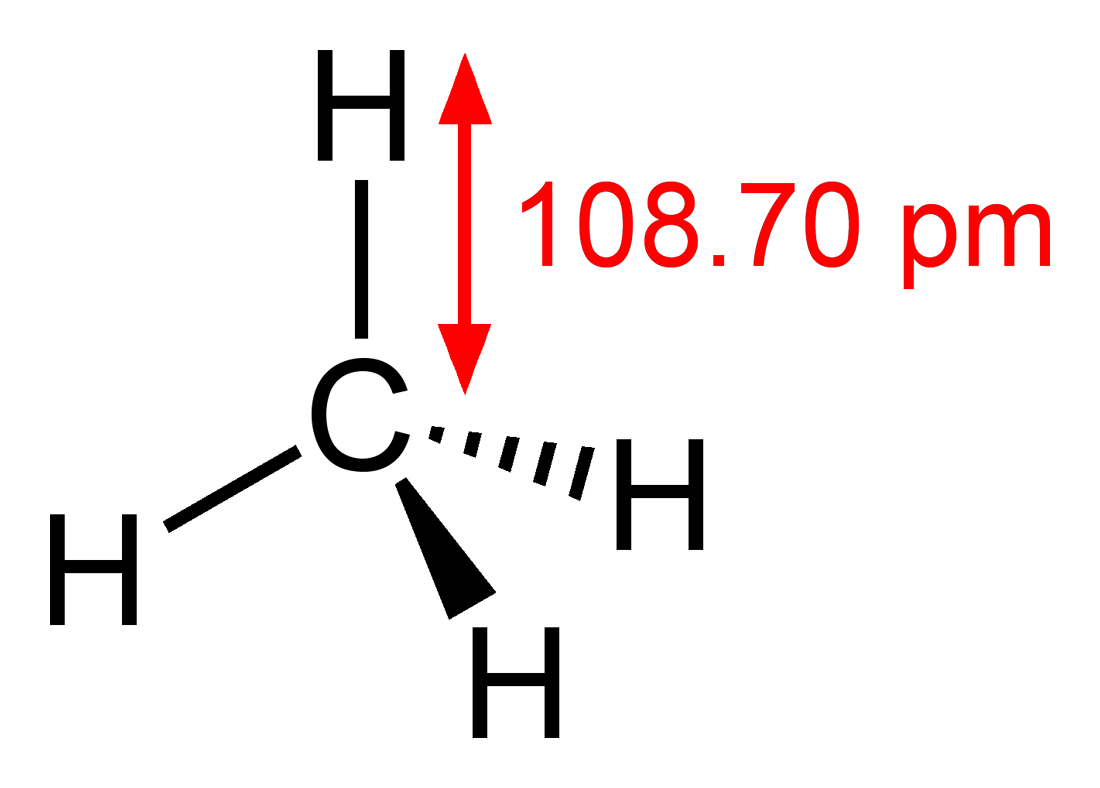
\includegraphics[width=0.4\textwidth]{metano.png}\\
\begin{itemize}
\item Las posiciones de los átomos  de metano $(CH_4)$ respecto a su centro de masas son:\\
 $\vec r_C = 0\, \vec x + 0 \, \vec y + 0 \, \vec z \, MeV^{-1}$\\
 $\vec r_{H1} = 0\, \vec x+0 \, \vec y + 550.87 \, \vec z \, MeV^{-1}$\\
 $\vec r_{H2} = 0\, \vec x -477.1 \, \vec y + -275.4\, \vec z \, MeV^{-1}$\\
 $\vec r_{H3} = 413.2\, \vec x + 238.5 \, \vec y + -272.4 \, \vec z \, MeV^{-1}$\\
 $\vec r_{H4} = -413.2 \, \vec x -238.5 \, \vec y + -272.4 \, \vec z \, MeV^{-1}$\\
 
\item Las masas de los átomos son\\
 $M_C = 11\, 187.97 \, MeV$\\
 $M_H = 938.272 MeV$\\
\end{itemize}
\end{frame}

%DIAPOSITIVA 13
\begin{frame}{Algunos ejemplos}
 A partir de estos datos construimos el tensor de inercia
 $$ \tilde I =
 \begin{pmatrix}
 818.6 & 0 & 0 \\
 0 & 818.6 & 0 \\
 0 & 0 & 640.7\\
 \end{pmatrix}
 \, eV^{-1}
 $$
 
Esta molécula se comporta trompo simétrico alargado

Su energía rotacional es
 $$E_{rot}=[6.1\cdot 10^{-3}J(J+1) -1.6 \cdot 10^{-3}K^2] \, eV$$
\end{frame}

%DIAPOSITIVA 14
\begin{frame}{Aproximación de los estados vibracionales}
\framesubtitle{Un poco de mecánica clásica}
\begin{itemize}
\item Suponemos N masas puntuales (los núcleos) cada uno de los cuales vibra en torno a una posición de equilibrio.
\item La energía cinética clásica de vibración en torno a la posición de equilibrio es:
\begin{equation}
T= \frac{1}{2}\sum_{\alpha = 1}^Nm_\alpha\left[\left(\frac{dx_\alpha}{dt}\right)^2+\left(\frac{dy_\alpha}{dt}\right)^2+\left(\frac{dz_\alpha}{dt}\right)^2\right]
\end{equation}
en coordenadas ponderadas
\begin{equation}
T=\frac{1}{2}\sum_{i=1}^{3N}\dot q_i^2
\end{equation}
\item La energía potencial en torno al equilibrio es:
\begin{equation}
U = U_e + \frac{1}{2}\sum_{i=1}^{3N}\sum_{k=1}^{3N}\left(\frac{\partial^2U}{\partial q_i \partial q_k}\right)_eq_iq_k
\end{equation}
\end{itemize}
\end{frame}

%DIAPOSITIVA 15
\begin{frame}
\begin{itemize}
\item En forma matricial
\begin{equation}
T=\frac{1}{2}\boldsymbol {\dot q}^t\boldsymbol {\dot q}
\end{equation}
\begin{equation}
U=U_e+\frac{1}{2}\boldsymbol q^t\tilde U\boldsymbol q
\end{equation}
\item Diagonalizamos $\tilde U$.
\begin{equation}
\tilde L^t\tilde U\tilde L = \tilde \Lambda
\end{equation}
\item Definimos las coordenadas normales $Q_i$ como:
\begin{equation}
\boldsymbol Q = \tilde L^t\boldsymbol q \Rightarrow \boldsymbol q = \tilde L\boldsymbol Q
\end{equation}
\item Nos queda
\begin{equation}
U-U_e=\frac{1}{2}\boldsymbol q^t\tilde U \boldsymbol q = \frac{1}{2}\boldsymbol Q^t (\tilde L^t\tilde U \tilde L) \boldsymbol Q =  \frac{1}{2}\boldsymbol Q^t\tilde \Lambda \boldsymbol Q
\end{equation}
\begin{equation}
T=\frac{1}{2}\boldsymbol{\dot q^t \dot q}=\frac{1}{2}\boldsymbol{\dot Q}\tilde L^t\tilde L\boldsymbol{\dot Q}= \frac{1}{2}\dot{\boldsymbol Q^t}\dot{\boldsymbol Q}
\end{equation}
\end{itemize}
\end{frame}

%DIAPOSITIVA 16
\begin{frame}
\begin{itemize}
\item El hamiltoniano queda:
\begin{equation}
\hat H= \frac{1}{2}\sum_{k=1}^{3N-6} \hat{\dot Q}_k^2 + \frac{1}{2} \sum_{k=1}^{3N-6} \lambda_k \hat Q_k^2 + U_e
\end{equation}
{\tiny Con $\lambda_k$ los autovalores de $\tilde \Lambda$}
\item $\lambda_{N-5}=...=\lambda_N=0$ corresponden a los grados de libertad traslacionales y rotacionales.
\item Teniendo en cuenta que $p_x=m\dot x$ nos queda 
\begin{equation}
\hat{\dot{Q_k}}=\frac{\hbar}{i}\frac{\partial}{\partial Q_k}
\end{equation}
\item Luego tomando $U_e=0$ el hamiltoniano final es
\begin{equation}
\hat H= -\frac{\hbar^2}{2}\sum_{k=1}^{3N-6} \frac{\partial^2}{\partial Q^2_k} + \frac{1}{2} \sum_{k=1}^{3N-6} \lambda_k \hat Q_k^2
\end{equation}
\end{itemize}
\end{frame}

%DIAPOSITIVA 17
\begin{frame}
\begin{itemize}
\item El hamiltoniano es separable: $\hat H=\displaystyle\sum_{k=1}^{2N-6} \hat H_k$ con
\begin{equation}
\hat H_k = -\frac{\hbar^2}{2}\frac{\partial^2}{\partial Q^2}+\frac{1}{2}\lambda_kQ_k^2
\end{equation}
que tiene la estructura del oscilador armónico, cuyas soluciones ya conocemos:
\begin{equation}
\psi_k(Q_k)\frac{1}{\left(2^{v_k}v_k!\right)^{1/2}}\left(\frac{\alpha_k}{\pi}\right)^{1/4}e^{-\alpha_kQ^2_k/2}H_{v_k}(\alpha_k^{1/2}Q_k)
\end{equation}
\begin{equation}
E_k=\left(v_k+\frac{1}{2}\right)h\nu_k,	\qquad v_k=0,1,2,...
\end{equation}
\begin{equation}
\alpha_k=\frac{2\pi\nu_k}{\hbar}=\frac{\lambda_k^{1/2}}{\hbar} \qquad \nu_k=\lambda_k^{1/2}
\end{equation}
\end{itemize}
\end{frame}

%DIAPOSITIVA 18
\begin{frame}{Obtención de los autoestados y autovalores en general}
\begin{itemize}
\item En genergal, para una molécula poliatómica el hamiltoniano estará constituido por:
\begin{itemize}
\item La energía cinética del movimiento de los núcleos
\item La energía cinética de los electrones
\item La interacción electrostática entre núcleos, entre electrones, y entre núcleos y electrones
\end{itemize}
$$
\hat H = -\frac{\hbar^2}{2}\sum_{\alpha=1}\frac{\nabla_\alpha^2}{m_\alpha}-\frac{\hbar^2}{2m}\sum_{i}\nabla_i^2+\sum_\alpha\sum_{\beta >\alpha}\frac{Z_\alpha Z_\beta e^2}{r_{\alpha \beta}}
$$
\begin{equation}
-\sum_\alpha\sum_i\frac{Z_\alpha e^2}{r_{i\alpha}}+\sum_j\sum_{i>j}\frac{e^2}{r_{ij}}
\end{equation}
\item Aproximación de Born-Oppenheimer. Separamos el movimiento electrónico del movimiento de los núcleos
\begin{equation}
\hat H_{el} = -\frac{\hbar^2}{2m}\sum_{i}\nabla_i^2-\sum_\alpha\sum_i\frac{Z_\alpha e^2}{r_{i\alpha}}+\sum_j\sum_{i>j}\frac{e^2}{r_{ij}}
\end{equation}
\end{itemize}
\end{frame}

%DIAPOSITIVA 19
\begin{frame}{Obtención de los autoestados y autovalores en general}
\begin{itemize}
\item Una vez obtenida la energía  electrónica $E_{el}$ podemos escribir el hamiltoniano nuclear
\begin{equation}
\hat H_N=-\frac{\hbar^2}{2}\sum_\alpha \frac{\nabla^2_\alpha}{m_\alpha}+V_{NN}+E_{el}
\end{equation}
\item Para una molécula diatómica, llamando $U(q_\alpha)\equiv E_{el}+V_{NN}$, escribiendo la ecuación en coordenadas del centro de masas y excluyendo la energía translacional nos queda:
\begin{equation}
\left[-\frac{\hbar^2}{2\mu}\nabla^2+U(R)\right]\psi_N=E\psi_N
\end{equation}
\item Tenemos un problema de fuerzas centrales
\begin{equation}
\psi_N=F(R)Y^M_J(\theta_N,\phi_N)
\end{equation}
\end{itemize}
\end{frame}

%DIAPOSITIVA 20
\begin{frame}{Obtención de los autoestados y autovalores en general}
\begin{itemize}
\item El potencial U(R) se encuentra resolviendo la ecuación electrónica molecular de Schrodinger
\item Buscamos una aproximación que represente razonablemente bien este potencial para la mayoría de las moléculas
\item Esperamos que el núcleo vibre alrededor de un mínimo de potencial de enrgía
\begin{equation*}
U(R) \approx U(R_e)+\frac{1}{2}U''(R_e)(R-R_e)^2
\end{equation*}
\item Con algunos cambios de variables ($G(R)=RF(R), \,\ q=R-R_e$) y desarrollando el laplaciano:
\begin{equation*}
-\frac{\hbar^2}{2\mu}G''(q)+\left[\frac{J(J+1)\hbar^2}{2\mu (q+R_e)^2}+U(R_e)+\frac{1}{2}k_eq^2-E\right]G(q)=0
\end{equation*}
\end{itemize}
\end{frame}

%DIAPOSITIVA 21
\begin{frame}{Obtención de los autoestados y autovalores en general}
\begin{itemize}
\item Otra aproximación
\begin{equation*}
\frac{J(J+1)\hbar^2}{2\mu (q+R_e)^2}=\frac{J(J+1)\hbar^2}{2\mu R_e^2}\left[1-2\frac{q}{R_e}+3\frac{q^2}{R_e^2}-...\right] \approx \frac{J(J+1)\hbar^2}{2\mu R_e^2}
\end{equation*}
\item Llamando
\begin{equation*}
W \equiv	E-U(R_e)-\frac{J(J+1)\hbar^2}{2\mu R_e^2}
\end{equation*}
\item Llegamos al oscilador armónico
\begin{equation}
-\frac{\hbar^2}{2\mu}G''(q)\left[\frac{1}{2}k_eq^2-W\right] G(q)=0
\end{equation}
Y la energía final es
\begin{equation}
E=U(R_e)+\left(v+\frac{1}{2}\right)h\nu_e+J(J+1)hB_e
\end{equation}
\end{itemize}
\end{frame}

%DIAPOSITIVA 22
\begin{frame}{Obtención de los autoestados y autovalores en general}
\begin{itemize}
\item Por tanto:
\begin{equation}
E_{tot} = U_e+E_{vib}+E_{rot}+E_{trans}
\end{equation}
\begin{equation}
\psi=\psi_{el}\psi_{vib}\psi_{rot}\psi_{trans}
\end{equation}
\end{itemize}

\end{frame}
\end{document}